\documentclass{article}

% XeLaTeX
\usepackage{xltxtra}
\usepackage{xunicode}
\usepackage{listings}
\usepackage[landscape]{geometry}

% Fonts
\setmainfont{DejaVu Sans} %{Arial}
\newfontfamily\cyrillicfont{Nimbus Roman No9 L} %{Arial}
\setmonofont{Courier New}
%\setmonofont{Ubuntu Mono}

%\setmonofont{DejaVu Sans Mono}

% Lang
\usepackage{polyglossia}
\setmainlanguage{russian}
\setotherlanguage{english}
\usepackage[dvipsnames,table]{xcolor}


\ifx\pdfoutput\undefined
\usepackage{graphicx}
\else
\usepackage[pdftex]{graphicx}
\fi

\lstset{
	language=python,
	keywordstyle=\color{Emerald},%\texttt, 
	commentstyle=\color{OliveGreen},%\texttt,
	stringstyle=\color{Bittersweet},%\texttt,
	tabsize=4,
	numbers=left,
	xleftmargin=10pt,
	morekeywords={with,as},	
	numberstyle=\large,
	%identifierstyle=\texttt,
	%basicstyle=\texttt,
}

\usepackage{hyperref}

\hypersetup{
	colorlinks=true,
	urlcolor=blue
}

\usepackage{float}
%\floatstyle{boxed} 
%\restylefloat{figure}
\usepackage[normalem]{ulem}


\begin{document}
\LARGE

%-------------------------------------------------------------------------------

{
\LARGE \vspace{15pt}
\begin{lstlisting}
	def read_message(socket):
		uname = socket.recv(NAME_SIZE)
		res = Result(uname)
		input_msg = socket.recv(INPUT_MSG_SIZE)
		while "BYE!" != input_msg:
			res.add_message(input_msg)
			input_msg = socket.recv(INPUT_MSG_SIZE)

		return res
\end{lstlisting}
}

\newpage

%-------------------------------------------------------------------------------
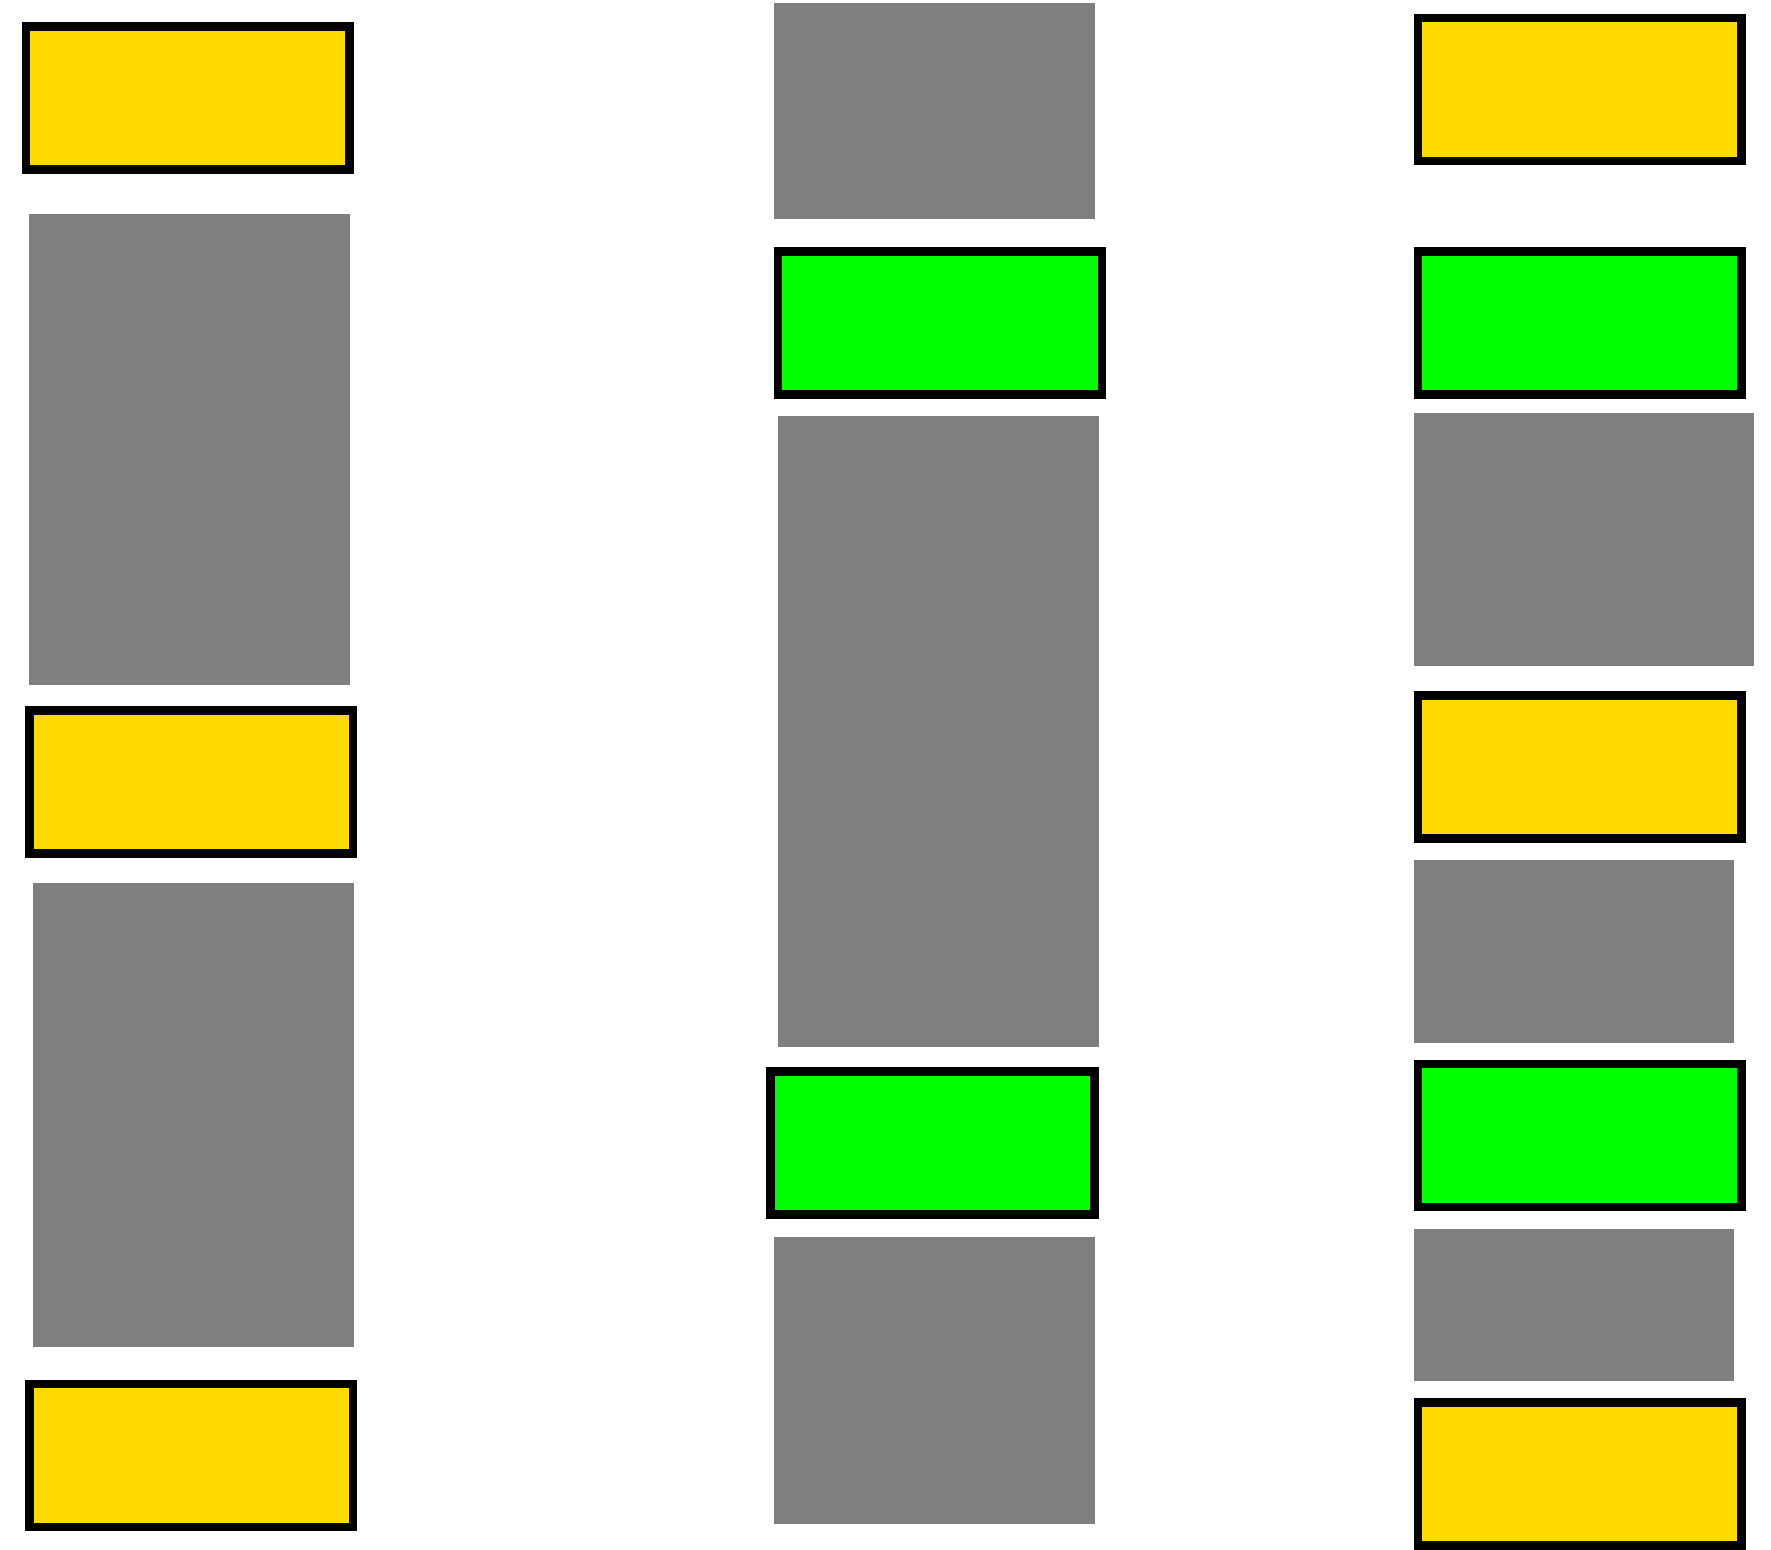
\includegraphics[scale=0.4]{images/threads.pdf}
\newpage
%-------------------------------------------------------------------------------
\center{10K problem}
\begin{itemize}
\item http://www.kegel.com/c10k.html
\item Много времени на переключение в ядро и назад
\item Алгоритм шедулера в ядре не совсем подходит для таких задач
\item На самом деле решение ближе к кооперативной многозадачности
\end{itemize}

\newpage
%-------------------------------------------------------------------------------
\center{select + конечные автоматы}
{
\LARGE \vspace{15pt}
\begin{lstlisting}
	import select
	r_rd, w_rd, e_rd = select.select(
				read_fds, write_fds, err_fds, timeout=0)

	pobj = select.poll()
	pobj.register(fd, EVENT_TYPE)
	...

	fd_end_evts = pobj.poll(timeout=0)
\end{lstlisting}
}
\newpage
%-------------------------------------------------------------------------------
\center{Async libs}
\begin{itemize}
	\item переписываем наш код из хороших и понятных последовательных 
			функций на ужасные конечные автоматы
	\item регистрируем обработчики событий функции или классы
	\item запускаем цикл обработки событий
	\item по мере продвижения обработки запроса одни функции регистрируют другие в качестве "продолжателей дела"
	\item базовые классы для разных протоколов способны облегчить ситуацию
	\item Но их на всех не хватит
\end{itemize}
\newpage
%-------------------------------------------------------------------------------
{
\Large \vspace{15pt}
\begin{lstlisting}

	def new_request(socket):
		return read_name, Result()

	def read_name(data, res):
		if len(data) >= NAME_SIZE - len(res.name):
			res.name += data[:NAME_SIZE - len(res.name)]
			return read_message(data[NAME_SIZE - len(res.name):], res)
		else:
			res.name += data
			return read_name, res

	def read_message(data, res):
		#....
		if message == "BYE!":
			save(res)
			return CLOSE_CONN
		else:
			#....
		return read_message, res

	def conn_closed(res):
		pass

	io_loop.register(new_request, port=15678, proto=TCP)
	io_loop.run()

\end{lstlisting}
}
\newpage
%-------------------------------------------------------------------------------
{
\Large \vspace{15pt}
\begin{lstlisting}
	from twisted.internet import reactor, protocol
	from twisted.protocols import basic

	class PubProtocol(basic.LineReceiver):
	    def __init__(self, factory):
	        self.factory = factory

	    def connectionMade(self):
	        self.factory.clients.add(self)

	    def connectionLost(self, reason):
	        self.factory.clients.remove(self)

	    def lineReceived(self, line):
	        for c in self.factory.clients:
	            c.sendLine("<{}> {}".format(self.transport.getHost(), line))

	class PubFactory(protocol.Factory):
	    def __init__(self):
	        self.clients = set()

	    def buildProtocol(self, addr):
	        return PubProtocol(self)

	reactor.listenTCP(1025, PubFactory())
	reactor.run()
\end{lstlisting}
}	
\newpage
%-------------------------------------------------------------------------------
\center{Генераторы. Cogen}
{
\Large \vspace{15pt}
\begin{lstlisting}
	class SocketWrapper(object):
		def __init__(self, real_socket):
			self.real_socket = real_socket

		def recv(self, sz):
			return "READ", self.real_socket, sz

		def send(self, data):
			return "SEND", self.real_socket, data

	def read_message(socket):
		uname = yield socket.recv(NAME_SIZE)
		res = Result(uname)
		input_msg = yield socket.recv(INPUT_MSG_SIZE)
		while "BYE!" != input_msg:
			res.add_message(input_msg)
			input_msg = yield socket.recv(INPUT_MSG_SIZE)

		return res
\end{lstlisting}
}	
\newpage
%-------------------------------------------------------------------------------
\center{Генераторы. Twisted}
{
\Large \vspace{15pt}
\begin{lstlisting}
	from twisted.internet import reactor, protocol, defer, endpoints
	from twisted.mail import imap4
	from twisted.python import log, failure

	@defer.inlineCallbacks
	def main(username="alice", password="secret",
	         strport="ssl:host=example.com:port=993"):
	    endpoint = endpoints.clientFromString(reactor, strport)
	    factory = protocol.Factory()
	    factory.protocol = imap4.IMAP4Client
	    try:
	        client = yield endpoint.connect(factory)
	        yield client.login(username, password)
	        yield client.select('INBOX')
	        info = yield client.fetchEnvelope(imap4.MessageSet(1))
	        print info[1]['ENVELOPE'][1]
	    except:
	        log.err(failure.Failure(), "IMAP4 client interaction failed")
	    reactor.stop()

	import sys
	main(*sys.argv[1:])
	reactor.run()
\end{lstlisting}
}	
\newpage

%-------------------------------------------------------------------------------
\center{gevent, eventlet, ..}
\begin{itemize}
	\item http://www.gevent.org/
	\item greenlet (part of stackless python spin-off)
	\item libev inside (c)
	\item Хак для создания легковесных python потоков в пользовательском режиме
	\item Автоматически сохраняет состояние точки 
			исполнения при запросе блокирующей операции и передает управление
			  циклу обработки
	\item ОС пользовательского режима с кооперативной многозадачностью
	\item \lstinline!from gevent import monkey; monkey.patch_socket()! и снова пишем нормальный код
	\item http://nichol.as/benchmark-of-python-web-servers
\end{itemize}
\newpage
%-------------------------------------------------------------------------------
\center{gevent, eventlet, ..}
{
\Large \vspace{15pt}
\begin{lstlisting}
	import gevent
	from gevent import monkey
	monkey.patch_all()

	import urllib2

	def print_head(url):
	    data = urllib2.urlopen(url).read()
	    print ('%s: %s bytes: %r' % (url, len(data), data[:50]))

	urls = ['http://www.google.com', 
			'http://www.yandex.ru', 
			'http://www.python.org']

	jobs = [gevent.spawn(print_head, url) for url in urls]

	gevent.joinall(jobs)
\end{lstlisting}
}
\newpage
%-------------------------------------------------------------------------------
\center{tornado}
%-------------------------------------------------------------------------------
\center{ДЗ}
\begin{flushleft}
Написать RPC сервер и клиент к нему.
API для сервера:
\begin{lstlisting}
c = RPCServer(ip, port)

def func1(x,y,z):
	return x + y ** z

# can register any amount of any functions
c.register(func1)
c.register(func2)

c.run()
\end{lstlisting}

API для клиента:
\begin{lstlisting}
c = RPCClient(api, port)

print c.func1(1, 2, 3) # напечатает 9
\end{lstlisting}

pickle, marshal, exec и eval  забаненны.
На всякий случай - все параметры и имя функции нужно передать на сервер, 
там вызвать зарегистрированную функцию, получить ее результат и отдать его на клиент.
Если функция с запрошенным именем не зарегистрированна или при ее 
исполнении произошла ошибка - передать сообщение на клиент и выбросить там исключение.
Необходимо поддерживать следующие типы данных: str, int, list.
Данные передавать через tcp сокеты. \\

Бонус:

\begin{itemize}
\item Поддерживать мапы и пользовательские классы
\item сделать так, что-бы на клиенте можно было получить имена функций питоновским способом
\item сделать так, что-бы клиенткий объект имел поля-функции, 
      полностью имитирующие функции на сервере.
      Для этого можно использовать eval, но нужно провести полную 
      валидацию строки, которая будет переданна в eval,
      для исключения возможности исполнения вредоносного кода при ее вызове.
\item Сделать 3 варинта сервера - на потоках (на каждый запрос порождать новый), 
    на пуле потоков и на gevent,
    сравнить производительность этих решений и объемы ресурсов в 
    зависимости от количества клиентов.
\end{itemize}
\end{flushleft}
%-------------------------------------------------------------------------------
\end{document}


